\documentclass[a4paper,10pt]{article}
\usepackage[utf8]{inputenc}
\usepackage[T1]{fontenc}
\usepackage{amsmath,amssymb}
\usepackage{graphicx}
\usepackage[table]{xcolor}
\usepackage{tikz}
\usepackage{tabularx}
\usepackage{hyperref}
\usepackage[margin=1.5cm]{geometry}

\title{\textcolor{blue}{DocStruct Stress Test}}
\author{\textcolor{red}{Comprehensive PDF Feature Test}}
\date{\today}

\begin{document}

\maketitle

\section{\textcolor{green!60!black}{Mixed Content Overview}}

This document is designed to \textbf{stress test} the \textit{DocStruct} pipeline with:
\textcolor{purple}{colored text}, \underline{underlined text}, and \textsf{different fonts}.

\subsection{Mathematical Equations}

Inline math: $E = mc^2$, $\alpha + \beta = \gamma$, $\int_0^\infty e^{-x^2} dx = \frac{\sqrt{\pi}}{2}$

\textcolor{orange}{Display equations with colors:}

\begin{equation}
\textcolor{red}{f(x)} = \sum_{n=0}^{\infty} \frac{x^n}{n!} = e^x
\end{equation}

\begin{equation}
\textcolor{blue}{\nabla \times \mathbf{E}} = -\frac{\partial \mathbf{B}}{\partial t}, \quad
\textcolor{green!60!black}{\nabla \cdot \mathbf{B}} = 0
\end{equation}

Matrix equation:
\[
\begin{bmatrix}
\textcolor{red}{a} & \textcolor{blue}{b} \\
\textcolor{green!60!black}{c} & \textcolor{orange}{d}
\end{bmatrix}
\begin{bmatrix}
x \\ y
\end{bmatrix}
=
\begin{bmatrix}
1 \\ 0
\end{bmatrix}
\]

\subsection{\textcolor{magenta}{Tables with Colors}}

\begin{table}[h]
\centering
\begin{tabular}{|l|c|r|}
\hline
\rowcolor{yellow!30}
\textbf{Feature} & \textbf{Value} & \textbf{Unit} \\
\hline
\textcolor{red}{Temperature} & 23.5 & °C \\
\hline
\rowcolor{cyan!20}
\textcolor{blue}{Pressure} & 101.3 & kPa \\
\hline
\textcolor{green!60!black}{Humidity} & 65 & \% \\
\hline
\rowcolor{orange!20}
\textcolor{purple}{Voltage} & 220 & V \\
\hline
\end{tabular}
\caption{\textcolor{brown}{Measurement data with colored rows}}
\end{table}

\subsection{Lists and Enumerations}

\textcolor{teal}{Unordered list:}
\begin{itemize}
    \item \textcolor{red}{Red item} with $\pi \approx 3.14159$
    \item \textcolor{blue}{Blue item} with $\sqrt{2} \approx 1.414$
    \item \textcolor{green!60!black}{Green item} with $\phi = \frac{1+\sqrt{5}}{2}$
\end{itemize}

\textcolor{violet}{Ordered list:}
\begin{enumerate}
    \item First: $\lim_{n \to \infty} (1 + \frac{1}{n})^n = e$
    \item Second: $\sum_{n=1}^{\infty} \frac{1}{n^2} = \frac{\pi^2}{6}$
    \item Third: $\int_{-\infty}^{\infty} e^{-x^2} dx = \sqrt{\pi}$
\end{enumerate}

\subsection{\textcolor{red!70!black}{Graphics and Diagrams}}

\begin{center}
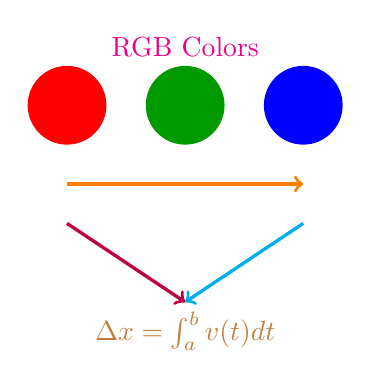
\begin{tikzpicture}
    % Colored circles
    \fill[red] (0,0) circle (0.5cm);
    \fill[green!60!black] (1.5,0) circle (0.5cm);
    \fill[blue] (3,0) circle (0.5cm);
    
    % Colored lines and arrows
    \draw[->,very thick,orange] (0,-1) -- (3,-1);
    \draw[->,very thick,purple] (0,-1.5) -- (1.5,-2.5);
    \draw[->,very thick,cyan] (3,-1.5) -- (1.5,-2.5);
    
    % Labels
    \node[above] at (1.5,0.5) {\textcolor{magenta}{RGB Colors}};
    \node[below] at (1.5,-2.5) {\textcolor{brown}{$\Delta x = \int_a^b v(t) dt$}};
\end{tikzpicture}
\end{center}

\subsection{Special Characters and Symbols}

Greek: $\alpha, \beta, \gamma, \delta, \epsilon, \zeta, \eta, \theta, \lambda, \mu, \nu, \xi, \pi, \rho, \sigma, \tau, \phi, \chi, \psi, \omega$

Math operators: $\sum, \prod, \int, \oint, \nabla, \partial, \infty, \forall, \exists, \in, \notin, \subset, \supset$

Arrows: $\leftarrow, \rightarrow, \Leftarrow, \Rightarrow, \leftrightarrow, \Leftrightarrow, \uparrow, \downarrow$

\textcolor{red!70!black}{Comparison:} $\leq, \geq, \neq, \approx, \equiv, \sim, \propto$

\subsection{\textcolor{blue!70!black}{Complex Equation Block}}

\begin{align}
\textcolor{red}{\frac{\partial u}{\partial t}} &= \textcolor{blue}{\alpha \frac{\partial^2 u}{\partial x^2}} \quad \text{(Heat equation)} \\
\textcolor{green!60!black}{\nabla^2 \psi} &= \textcolor{orange}{\frac{1}{c^2} \frac{\partial^2 \psi}{\partial t^2}} \quad \text{(Wave equation)} \\
\textcolor{purple}{i\hbar \frac{\partial}{\partial t} \Psi} &= \textcolor{cyan}{\hat{H} \Psi} \quad \text{(Schrödinger equation)}
\end{align}

\subsection{Hyperlinks}

Visit \textcolor{blue}{\href{https://github.com/zeetee1235/DocStruct}{DocStruct GitHub}} for more information.

\subsection{\textcolor{cyan!70!black}{Code Blocks}}

Python example with \textcolor{red}{syntax} and \textcolor{blue}{indentation}:

\begin{verbatim}
def factorial(n):
    """Calculate factorial recursively"""
    if n <= 1:
        return 1
    return n * factorial(n - 1)

# Test the function
print(f"5! = {factorial(5)}")  # Output: 120
\end{verbatim}

\textcolor{green!60!black}{Rust example}:

\begin{verbatim}
fn main() {
    let numbers = vec![1, 2, 3, 4, 5];
    let sum: i32 = numbers.iter().sum();
    println!("Sum: {}", sum);
}
\end{verbatim}

\vfill

\begin{center}
\fbox{\parbox{0.9\textwidth}{
\centering
\textcolor{red}{\textbf{End of Stress Test}} \\
\textcolor{blue}{This document contains: tables, equations, colors, graphics, lists, symbols, and hyperlinks.}
}}
\end{center}

\end{document}
